\chapter{第二代:自优化与遗传进化}
\label{chap:gen2}

\section{概述}

第二代在第一代基础上扩展了自优化能力、基于遗传算法的进化和实时测试。本章详细介绍了改进、实现策略和预期的性能提升。

\begin{figure}[h]
\centering
\begin{tikzpicture}[
    node distance=1.5cm,
    gen1/.style={rectangle, draw=blue!50, fill=blue!10, thick, minimum width=3cm, minimum height=1.5cm, text centered, rounded corners},
    gen2/.style={rectangle, draw=green!50, fill=green!10, thick, minimum width=3cm, minimum height=1.5cm, text centered, rounded corners},
    arrow/.style={->, >=stealth, thick, blue!70},
    label/.style={text width=2.5cm, text centered, font=\small}
]
    % Generation One
    \node[gen1] (gen1) {Generation One\\\small AI Generation\\Concurrent Testing};
    
    % Generation Two additions
    \node[gen2, right=of gen1] (selfopt) {Self\\Optimization};
    \node[gen2, below=of gen1] (genetic) {Genetic\\Evolution};
    \node[gen2, below=of selfopt] (onthefly) {On-the-Fly\\Testing};
    
    % Arrows showing evolution
    \draw[arrow] (gen1) -> node[above, label] {Enhanced with} (selfopt);
    \draw[arrow] (gen1) -> node[left, label] {Enhanced with} (genetic);
    \draw[arrow] (selfopt) -> node[right, label] {Works with} (onthefly);
    \draw[arrow] (genetic) -> node[below, label] {Works with} (onthefly);
    
    % Combined system
    \node[gen2, below=of onthefly, xshift=-1.5cm, minimum width=6.5cm, fill=green!20] (gen2system) {Generation Two\\Complete System};
    
    \draw[arrow] (selfopt) -> (gen2system);
    \draw[arrow] (genetic) -> (gen2system);
    \draw[arrow] (onthefly) -> (gen2system);
\end{tikzpicture}
\caption{从第一代到第二代的演进}
\label{fig:gen1-to-gen2}
\end{figure}

\section{关键改进}

\subsection{自优化系统}

\subsubsection{自适应参数调整}

系统根据成功率持续优化自身参数:

\begin{lstlisting}[language=Python, caption=自优化模块]
class SelfOptimizer:
    def __init__(self):
        self.parameter_history = []
        self.performance_history = []
        self.optimization_interval = 100  # Optimize every 100 simulations
        
    def optimize_parameters(self, current_performance: dict):
        """Optimize system parameters based on performance"""
        # Track current performance
        self.performance_history.append(current_performance)
        
        if len(self.performance_history) < self.optimization_interval:
            return  # Not enough data yet
        
        # Analyze performance trends
        recent_performance = self.performance_history[-self.optimization_interval:]
        avg_success_rate = np.mean([p['success_rate'] for p in recent_performance])
        avg_sharpe = np.mean([p['avg_sharpe'] for p in recent_performance])
        
        # Adjust parameters
        if avg_success_rate < 0.3:
            # Low success rate: increase exploration
            return {
                'exploration_rate': min(0.5, current_performance['exploration_rate'] * 1.2),
                'temperature': min(1.0, current_performance['temperature'] * 1.1),
                'mutation_rate': min(0.3, current_performance['mutation_rate'] * 1.15)
            }
        elif avg_success_rate > 0.6:
            # High success rate: increase exploitation
            return {
                'exploration_rate': max(0.1, current_performance['exploration_rate'] * 0.9),
                'temperature': max(0.5, current_performance['temperature'] * 0.95),
                'mutation_rate': max(0.05, current_performance['mutation_rate'] * 0.9)
            }
        else:
            # Maintain current parameters
            return current_performance
\end{lstlisting}

\subsubsection{Alpha质量时间跟踪}

监控Alpha性能退化:

\begin{lstlisting}[language=Python, caption=Alpha质量监控器]
class AlphaQualityMonitor:
    def __init__(self, monitoring_window: int = 30):
        self.monitoring_window = monitoring_window  # days
        self.alpha_history = {}  # {alpha_id: [performance_records]}
        
    def track_alpha(self, alpha_id: str, performance: dict):
        """Track alpha performance over time"""
        if alpha_id not in self.alpha_history:
            self.alpha_history[alpha_id] = []
        
        self.alpha_history[alpha_id].append({
            'timestamp': time.time(),
            'sharpe': performance['sharpe'],
            'fitness': performance['fitness'],
            'returns': performance['returns']
        })
        
        # Keep only recent history
        cutoff_time = time.time() - (self.monitoring_window * 24 * 3600)
        self.alpha_history[alpha_id] = [
            record for record in self.alpha_history[alpha_id]
            if record['timestamp'] > cutoff_time
        ]
    
    def detect_degradation(self, alpha_id: str) -> bool:
        """Detect if alpha performance is degrading"""
        if alpha_id not in self.alpha_history:
            return False
        
        history = self.alpha_history[alpha_id]
        if len(history) < 10:
            return False  # Not enough data
        
        # Calculate trend
        recent_sharpe = [r['sharpe'] for r in history[-10:]]
        older_sharpe = [r['sharpe'] for r in history[:-10]]
        
        if len(older_sharpe) > 0:
            recent_avg = np.mean(recent_sharpe)
            older_avg = np.mean(older_sharpe)
            
            # Degradation if recent performance is 20% worse
            if recent_avg < older_avg * 0.8:
                return True
        
        return False
    
    def get_alpha_health_score(self, alpha_id: str) -> float:
        """Calculate health score (0-1) for an alpha"""
        if alpha_id not in self.alpha_history:
            return 1.0  # New alpha, assume healthy
        
        history = self.alpha_history[alpha_id]
        if len(history) < 5:
            return 1.0
        
        # Calculate stability and trend
        sharpe_values = [r['sharpe'] for r in history]
        trend = np.polyfit(range(len(sharpe_values)), sharpe_values, 1)[0]
        stability = 1.0 / (1.0 + np.std(sharpe_values))
        
        # Health score combines trend and stability
        health = (stability * 0.6) + (max(0, 1.0 + trend) * 0.4)
        return min(1.0, max(0.0, health))
\end{lstlisting}

\subsection{遗传算法集成}

\subsubsection{Alpha进化系统}

通过交叉和变异进化成功的Alpha:

\begin{figure}[h]
\centering
\begin{tikzpicture}[
    node distance=1.2cm,
    parent/.style={rectangle, draw=blue!50, fill=blue!10, thick, minimum width=2.5cm, minimum height=1cm, text centered, rounded corners},
    child/.style={rectangle, draw=green!50, fill=green!10, thick, minimum width=2.5cm, minimum height=1cm, text centered, rounded corners},
    op/.style={circle, draw=orange!50, fill=orange!10, thick, minimum size=1cm, text centered, font=\small},
    arrow/.style={->, >=stealth, thick},
    label/.style={font=\small, text centered}
]
    % Parents
    \node[parent] (p1) at (-0.4cm,4.0cm) {Parent 1\\$ts\_rank(close, 20)$};
    \node[parent] (p2) at (5.6cm,4.0cm) {Parent 2\\$ts\_delta(volume, 1)$};
    
    % Crossover operation
    \node[op] (crossover) at (2.4cm,2.0cm) {Crossover};
    
    % Children after crossover
    \node[child] (c1) at (-2.8cm,0.0cm) {Child 1\\$ts\_rank(volume, 20)$};
    \node[child] (c2) at (8.8cm,0.0cm) {Child 2\\$ts\_delta(close, 1)$};
    
    % Mutation
    \node[op] (mut1) at (0.4cm,-2.0cm) {Mutate};
    \node[op] (mut2) at (5.6cm,-2.0cm) {Mutate};
    
    % Final offspring
    \node[child] (f1) at (-1.2cm,-5.2cm) {Offspring 1\\$ts\_rank(volume, 15)$};
    \node[child] (f2) at (6.4cm,-5.2cm) {Offspring 2\\$ts\_delta(close, 2)$};
    
    % Arrows
    \draw[arrow] (p1) -> (crossover);
    \draw[arrow] (p2) -> (crossover);
    \draw[arrow] (crossover) -> (c1);
    \draw[arrow] (crossover) -> (c2);
    \draw[arrow] (c1) -> (mut1);
    \draw[arrow] (c2) -> (mut2);
    \draw[arrow] (mut1) -> (f1);
    \draw[arrow] (mut2) -> (f2);
    
    % Labels
    \node[label, above=0.2cm of crossover] {Genetic Operations};
    \node[label, right=0.3cm of mut1] {Parameter\\Mutation};
\end{tikzpicture}
\caption{遗传算法:交叉与变异}
\label{fig:genetic-evolution}
\end{figure}

\begin{lstlisting}[language=Python, caption=Alpha进化的遗传算法]
class AlphaEvolutionEngine:
    def __init__(self, mutation_rate: float = 0.1, crossover_rate: float = 0.7):
        self.mutation_rate = mutation_rate
        self.crossover_rate = crossover_rate
        self.population = []  # Current population of alphas
        self.fitness_scores = {}  # {alpha_id: fitness_score}
        
    def initialize_population(self, initial_alphas: List[AlphaResult], 
                             population_size: int = 50):
        """Initialize population with successful alphas"""
        # Select top performers
        sorted_alphas = sorted(initial_alphas, 
                             key=lambda a: a.sharpe * a.fitness, 
                             reverse=True)
        self.population = sorted_alphas[:population_size]
        
        # Calculate fitness scores
        for alpha in self.population:
            self.fitness_scores[alpha.template] = (
                alpha.sharpe * 0.5 + alpha.fitness * 0.3 + 
                (1.0 / (1.0 + alpha.turnover)) * 0.2
            )
    
    def select_parents(self, num_parents: int = 2) -> List[str]:
        """Select parents using tournament selection"""
        parents = []
        tournament_size = 3
        
        for _ in range(num_parents):
            # Tournament selection
            tournament = random.sample(self.population, 
                                     min(tournament_size, len(self.population)))
            winner = max(tournament, 
                        key=lambda a: self.fitness_scores.get(a.template, 0))
            parents.append(winner.template)
        
        return parents
    
    def crossover(self, parent1: str, parent2: str) -> str:
        """Crossover two alpha expressions"""
        if random.random() > self.crossover_rate:
            return parent1  # No crossover
        
        # Parse expressions into trees
        tree1 = self.parse_expression(parent1)
        tree2 = self.parse_expression(parent2)
        
        # Select random subtree from each parent
        subtree1 = self.select_random_subtree(tree1)
        subtree2 = self.select_random_subtree(tree2)
        
        # Replace subtree in parent1 with subtree from parent2
        child = self.replace_subtree(tree1, subtree1, subtree2)
        
        return self.expression_to_string(child)
    
    def mutate(self, expression: str) -> str:
        """Mutate an alpha expression"""
        if random.random() > self.mutation_rate:
            return expression  # No mutation
        
        tree = self.parse_expression(expression)
        
        # Mutation operations
        mutation_type = random.choice([
            'replace_operator',
            'replace_field',
            'modify_parameter',
            'add_operator',
            'remove_operator'
        ])
        
        if mutation_type == 'replace_operator':
            # Replace an operator with another compatible one
            tree = self.replace_random_operator(tree)
        elif mutation_type == 'replace_field':
            # Replace a field with another from same category
            tree = self.replace_random_field(tree)
        elif mutation_type == 'modify_parameter':
            # Modify a numeric parameter
            tree = self.modify_random_parameter(tree)
        elif mutation_type == 'add_operator':
            # Add a new operator layer
            tree = self.add_random_operator(tree)
        elif mutation_type == 'remove_operator':
            # Remove an operator layer
            tree = self.remove_random_operator(tree)
        
        return self.expression_to_string(tree)
    
    def evolve_generation(self) -> List[str]:
        """Evolve one generation"""
        new_population = []
        
        # Elitism: keep top 10%
        elite_count = max(1, int(len(self.population) * 0.1))
        elite = sorted(self.population, 
                     key=lambda a: self.fitness_scores.get(a.template, 0),
                     reverse=True)[:elite_count]
        new_population.extend([a.template for a in elite])
        
        # Generate offspring
        while len(new_population) < len(self.population):
            # Select parents
            parents = self.select_parents(2)
            
            # Crossover
            child = self.crossover(parents[0], parents[1])
            
            # Mutate
            child = self.mutate(child)
            
            new_population.append(child)
        
        return new_population
\end{lstlisting}

\subsubsection{实时测试}

在生成过程中立即测试进化的Alpha:

\begin{lstlisting}[language=Python, caption=实时测试系统]
class OnTheFlyTester:
    def __init__(self, generator: EnhancedTemplateGeneratorV2):
        self.generator = generator
        self.test_queue = []
        self.test_results = {}
        
    def test_evolved_alpha(self, alpha_expression: str, region: str):
        """Test an evolved alpha immediately"""
        # Quick validation
        if not self.validate_expression(alpha_expression):
            return None
        
        # Submit quick test (shorter time period)
        settings = SimulationSettings(
            region=region,
            testPeriod="P1Y0M0D"  # 1 year instead of 5 years for speed
        )
        
        # Submit to test queue
        future = self.generator.simulate_template_concurrent(
            alpha_expression, region, settings
        )
        
        self.test_queue.append({
            'expression': alpha_expression,
            'region': region,
            'future': future,
            'timestamp': time.time()
        })
        
        return future
    
    def process_test_results(self):
        """Process completed test results"""
        completed = []
        for test in self.test_queue:
            if test['future'].done():
                try:
                    result = test['future'].result()
                    self.test_results[test['expression']] = result
                    completed.append(test)
                except Exception as e:
                    logger.error(f"Test failed: {e}")
        
        # Remove completed tests
        for test in completed:
            self.test_queue.remove(test)
        
        return len(completed)
    
    def get_fast_feedback(self, alpha_expression: str) -> dict:
        """Get quick feedback on alpha quality"""
        if alpha_expression in self.test_results:
            result = self.test_results[alpha_expression]
            return {
                'sharpe': result.sharpe,
                'fitness': result.fitness,
                'success': result.success,
                'quality': 'high' if result.sharpe > 1.5 else 
                          'medium' if result.sharpe > 1.25 else 'low'
            }
        return None
\end{lstlisting}

\section{预期改进}

\subsection{性能指标}

第二代预期实现:

\begin{figure}[h]
\centering
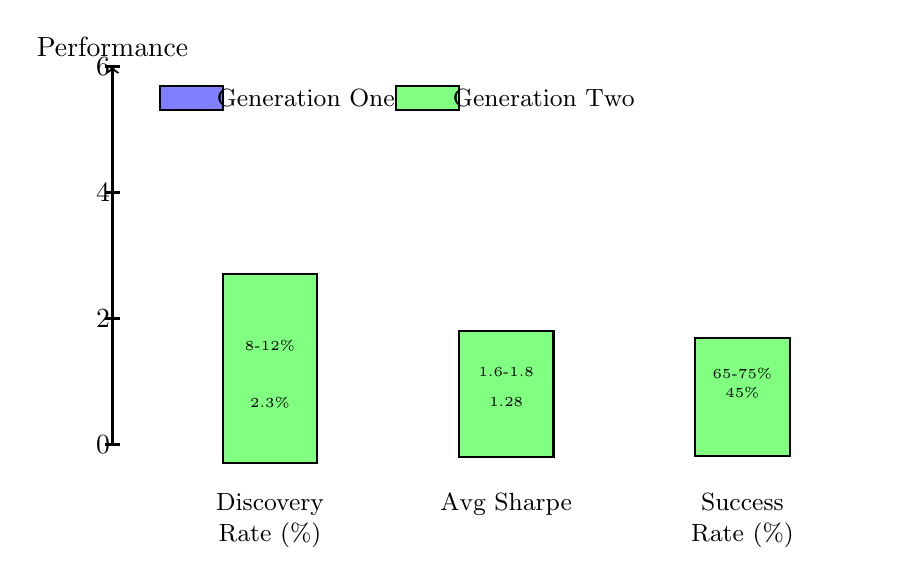
\begin{tikzpicture}[
    yscale=0.8,
    bar/.style={rectangle, draw, thick, minimum width=1.2cm, text centered, font=\small},
    gen1bar/.style={bar, fill=blue!50},
    gen2bar/.style={bar, fill=green!50},
    label/.style={font=\small, text width=3cm, text centered}
]
    % Y-axis
    \draw[->, thick] (0,0) -- (0,6) node[above] {Performance};
    \draw[thick] (-0.1,0) -- (0.1,0) node[left] {0};
    \draw[thick] (-0.1,2) -- (0.1,2) node[left] {2};
    \draw[thick] (-0.1,4) -- (0.1,4) node[left] {4};
    \draw[thick] (-0.1,6) -- (0.1,6) node[left] {6};
    
    % Metrics
    \node[label, below=0.5cm] at (2,0) {Discovery\\Rate (\%)};
    \node[label, below=0.5cm] at (5,0) {Avg Sharpe};
    \node[label, below=0.5cm] at (8,0) {Success\\Rate (\%)};
    
    % Generation One bars
    \node[gen1bar, minimum height=0.6cm] at (2,0.3) {};
    \node[gen1bar, minimum height=0.64cm] at (5,0.32) {};
    \node[gen1bar, minimum height=0.9cm] at (8,0.45) {};
    
    % Generation Two bars
    \node[gen2bar, minimum height=2.4cm] at (2,1.2) {};
    \node[gen2bar, minimum height=1.6cm] at (5,0.8) {};
    \node[gen2bar, minimum height=1.5cm] at (8,0.75) {};
    
    % Values
    \node[above=0.1cm] at (2,0.3) {\tiny 2.3\%};
    \node[above=0.1cm] at (2,1.2) {\tiny 8-12\%};
    \node[above=0.1cm] at (5,0.32) {\tiny 1.28};
    \node[above=0.1cm] at (5,0.8) {\tiny 1.6-1.8};
    \node[above=0.1cm] at (8,0.45) {\tiny 45\%};
    \node[above=0.1cm] at (8,0.75) {\tiny 65-75\%};
    
    % Legend
    \node[gen1bar, minimum height=0.3cm, minimum width=0.8cm] at (1,5.5) {};
    \node[right=0.2cm] at (1,5.5) {\small Generation One};
    \node[gen2bar, minimum height=0.3cm, minimum width=0.8cm] at (4,5.5) {};
    \node[right=0.2cm] at (4,5.5) {\small Generation Two};
\end{tikzpicture}
\caption{预期性能改进}
\label{fig:performance-improvements}
\end{figure}

\begin{table}[h]
\centering
\begin{tabular}{lcc}
\toprule
指标 & 第一代 & 第二代(预期) \\
\midrule
发现率 & 2.3\% & 8-12\% \\
平均Sharpe & 1.28 & 1.6-1.8 \\
成功率 & 45\% & 65-75\% \\
Alpha质量稳定性 & 不适用 & 30天内85\%+ \\
进化周期/小时 & 0 & 50-100 \\
\bottomrule
\end{tabular}
\caption{预期性能改进}
\end{table}

\subsection{关键优势}

\begin{enumerate}
    \item \textbf{自优化}:系统自动适应参数
    \item \textbf{遗传进化}:成功的Alpha进化并改进
    \item \textbf{实时测试}:进化过程中的即时反馈
    \item \textbf{质量监控}:跟踪Alpha随时间的退化
    \item \textbf{自适应学习}:系统从成功和失败中学习
\end{enumerate}

\section{实现策略}

\subsection{与第一代集成}

\begin{lstlisting}[language=Python, caption=第二代集成]
class EnhancedTemplateGeneratorV3(EnhancedTemplateGeneratorV2):
    """Generation Two: Extends Generation One with evolution"""
    
    def __init__(self, *args, **kwargs):
        super().__init__(*args, **kwargs)
        
        # Add Generation Two components
        self.self_optimizer = SelfOptimizer()
        self.evolution_engine = AlphaEvolutionEngine()
        self.quality_monitor = AlphaQualityMonitor()
        self.on_the_fly_tester = OnTheFlyTester(self)
        
        # Evolution parameters
        self.evolution_enabled = True
        self.evolution_interval = 50  # Evolve every 50 successful alphas
        self.evolution_count = 0
        
    def generate_and_evolve(self, regions: List[str], 
                           templates_per_region: int):
        """Generate templates with evolution"""
        results = []
        
        while True:
            # Generate new templates (Generation One)
            new_results = self.generate_and_test_templates(
                regions, templates_per_region, resume=True
            )
            results.extend(new_results)
            
            # Self-optimization
            if len(results) % 100 == 0:
                performance = self.calculate_performance_metrics(results)
                optimized_params = self.self_optimizer.optimize_parameters(
                    performance
                )
                self.apply_parameters(optimized_params)
            
            # Evolution
            if self.evolution_enabled and len(results) >= self.evolution_interval:
                successful_alphas = [r for r in results if r.success and r.sharpe > 1.25]
                
                if len(successful_alphas) >= 10:
                    # Initialize/evolve population
                    if self.evolution_engine.population == []:
                        self.evolution_engine.initialize_population(successful_alphas)
                    else:
                        # Evolve generation
                        evolved_expressions = self.evolution_engine.evolve_generation()
                        
                        # Test evolved alphas on-the-fly
                        for expr in evolved_expressions[:20]:  # Test top 20
                            for region in regions:
                                self.on_the_fly_tester.test_evolved_alpha(expr, region)
                        
                        self.evolution_count += 1
            
            # Quality monitoring
            for result in new_results:
                if result.success:
                    alpha_id = self.generate_alpha_id(result.template, result.region)
                    self.quality_monitor.track_alpha(alpha_id, {
                        'sharpe': result.sharpe,
                        'fitness': result.fitness,
                        'returns': result.returns
                    })
                    
                    # Check for degradation
                    if self.quality_monitor.detect_degradation(alpha_id):
                        logger.warning(f"Alpha {alpha_id} showing degradation")
\end{lstlisting}

\section{挑战与解决方案}

\subsection{计算复杂度}

\textbf{挑战}:遗传进化增加了计算负载。

\textbf{解决方案}:
\begin{itemize}
    \item 多个种群的并行进化
    \item 增量测试(仅测试有希望的变异)
    \item 表达式评估的缓存
\end{itemize}

\subsection{表达式有效性}

\textbf{挑战}:进化的表达式可能在语法上无效。

\textbf{解决方案}:
\begin{itemize}
    \item 基于语法的变异(仅有效操作)
    \item 测试前验证
    \item 无效表达式的修复机制
\end{itemize}

\section{总结}

第二代引入了:
\begin{itemize}
    \item 自优化参数调整
    \item 基于遗传算法的Alpha进化
    \item 实时测试以获取即时反馈
    \item 随时间变化的质量监控
    \item 从性能数据中自适应学习
\end{itemize}

这些改进预期将显著提高发现率和Alpha质量,同时保持系统稳定性。
